\documentclass[12pt, a4paper]{article}
\usepackage{import}
\usepackage{preamble}

\title{Cosmic Expansion MCMC}
\date{\(5^\mathrm{{th}}\) January 2023}
\author{Lee Farrugia}

\begin{document}
    
\maketitle
\thispagestyle{titlepagestyle}
\pagestyle{mystyle}

\section{Abstract}


\section{Introduction \& Theoretical Background}

In a binary system when one or both of the stars are white dwarves, one can observe a Supernovae type 1A. This happens when the white dwarf or in the case of two white dwarves, the larger white dwarf start to acquire matter from the other star to reach the Chandrasekhar limit. At this limit the star collapses. As the star reaches the Chandrasekhar limit, its nuclear fusion restarts and start fusing carbon into oxygen. In the las few moments of the star, its temperature reaches billions of Kelvins and due to the high energy it unbinds and releases a shock-wave that produces the supernovae. As this process can occur for any white dwarf, they all produce similar light curves, thus, we can use the supernovae type 1A as a standard candle in order to determine the distance modulus. Using this information one can determine the distance modulus of the data set provided by SN data.

\section{Materials \& Methods}
    \subsection{Language and Packages}

        Python 3.10.8, Numpy, Sympy, Scipy.integrate, Scipy.optimize, Matplotlib.pyplot, Pandas, Batman, Emcee, Corner, SN Dataset\,.

    \subsection{Methodology}

        \begin{enumerate}
            \item In order to obtain a plot for the \(\mathrm{\Lambda}\)CDM model the P18 parameter values for \(\mathrm{\Omega}_{\mathrm{matter}}\) and H\(_0\) and their uncertainties provided, for a range of redshift between 0 and 2.3\,.
            \item By numerically solving for the luminosity distance and using the P18 parameters, plot the luminosity distance for the same redshift range as before. By calculating the distance modulus using th SN dataset, plot the distance modulus against the redshift values in the dataset.
            \item Utilizing the MCMC method found in the emcee package determine the best fit parameters for the SN dataset. The number of walkers should be between 50 and 100, while the number of iterations should be between 10000 and 60000. Further more the initial states for \(H_0, \mathrm{\Omega}_{\mathrm{matter_0}}\) and \(M\) should be \(70, 0.3, -19\) respectively.
        \end{enumerate}

\section{Results \& Discussion}

As the core task was to determine the best fit parameters for the following equation:
\begin{equation}
    \mu = 5\log_{10}[d_L]+25+M\,,
    \label{eq:mu~equation}
\end{equation}
The first step to determine the best fit parameters for equation~\ref{eq:mu~equation}, the P18 parameters where used for a range of redshift starting from \qty{0}{km.s^{-1}} to \qty{2.3}{km.s^{-1}} with a step of \qty{0.1}{km.s^{-1}} each time. In order to calculate \(H(z)\) the \(\mathrm{\Lambda}\)CDM mode was used which provided the following equation:
\begin{equation}
    H(z)^2 = H_0^2[\Omega_{\mathrm{matter_0}}(1+z)^3+(1-\Omega_{\mathrm{matter_0}})]\,,
    \label{eq:Hz~equation}
\end{equation}

\begin{figure}[H]
    \centering
    \includegraphics[width = 0.7\textwidth]{Graph 1.png}
    \label{fig:Hz~vs~redshift}
\end{figure}

where \textit{H(z)} is the Hubble parameter in terms of the redshift, z is the redshift value and \(\Omega_{\mathrm{matter_0}}\) is the density parameter of matter in the Universe. The equation used is also called the Friedmann equation. The parameters used to calculate \(H(z)\) were \(H_0^{P18} = 67.4 \pm 0.5\) \unit{km.m.s^{-1}.Mpc^{-1}} and \(\Omega_{\mathrm{matter_0}} = 0.315 \pm 0.007\). This resulted in figure~\ref{fig:Hz~vs~redshift}, where one can clearly see that with a larger redshift it results in a larger value of \(H(z)\). The observed fit correlates with the graphs observed in \parencite{hubble}. The next step was to obtain the luminosity distance for the redshift range mentioned before. The luminosity distance was obtained using the following equation:

\begin{equation}
    d_L(z_i) = c(1+z_i)\\int_{0}^{z_i} \frac{dz'}{H(z')}\,,
    \label{eq:luminosity~distance}
\end{equation}

where \(d_L(z_i)\) is the luminosity distance, c is the speed of light taken as \qty{299792.458}{km.s^{-1}}, \(z_i\) is the redshift value. After numerically solving equation~\ref{eq:luminosity~distance}, figure \ref{fig:luminosity~vs~redshift} was obtained.

\begin{figure}[H]
    \centering
    \includegraphics[width = 0.7\textwidth]{Graph 2.png}
    \label{fig:luminosity~vs~redhsift}
\end{figure}

One should note that the luminosity distance decreases with redshift. This correlates with what is discussed in \parencite{pettiniHUBBLEDIAGRAMTYPE}, that is that the distance luminosity decreases with luminosity. Next the \(\mathrm{SN_data}\) was loaded into the program and a graph of the distance modulus against the redshift was plotted and can be seen in figure \ref{fig:distance~modulus~vs~redshift~sn}.

\begin{figure}[H]
    \centering
    \includegraphics[width = 0.7\textwidth]{Graph 3.png}
    \label{fig:distance~modulus~vs~redshift~sn}
\end{figure}

It should be noted that the date for the redshift did not have any errors where as the data for the distance modulus did have some uncertainties related to it which was duly added to the plotting parameters. It should also be noted that the distance modulus increases with the redshift. In order to obtain the best fit parameter for the \(\mathrm{SN_data}\) set the Markov Chain Monte Carlo method was used, abbreviated to MCMC. This is as the MCMC method allow for multiple iterations to obtain the best parameters to fit the data provided utilizing an initial positional value. For this experiment the initial positions were provided to be \(H_0\) = \qty{70}{km.s^{-1}.Mpc^{-1}}, \(\Omega_{\mathrm{matter_0}} = 0.3\) and \(M=-19\). Furthermore, the MCMC was set first use 100 walkers that are allowed to move randomly in the 3 dimensions. A sample of 2000 iteration was taken and using this sample the full computation of 60000 iterations was done in order to obtain the best fit parameters and the corner plot that can be seen in figure~\ref{fig:corner~plots}. 

\begin{figure}[H]
    \centering
    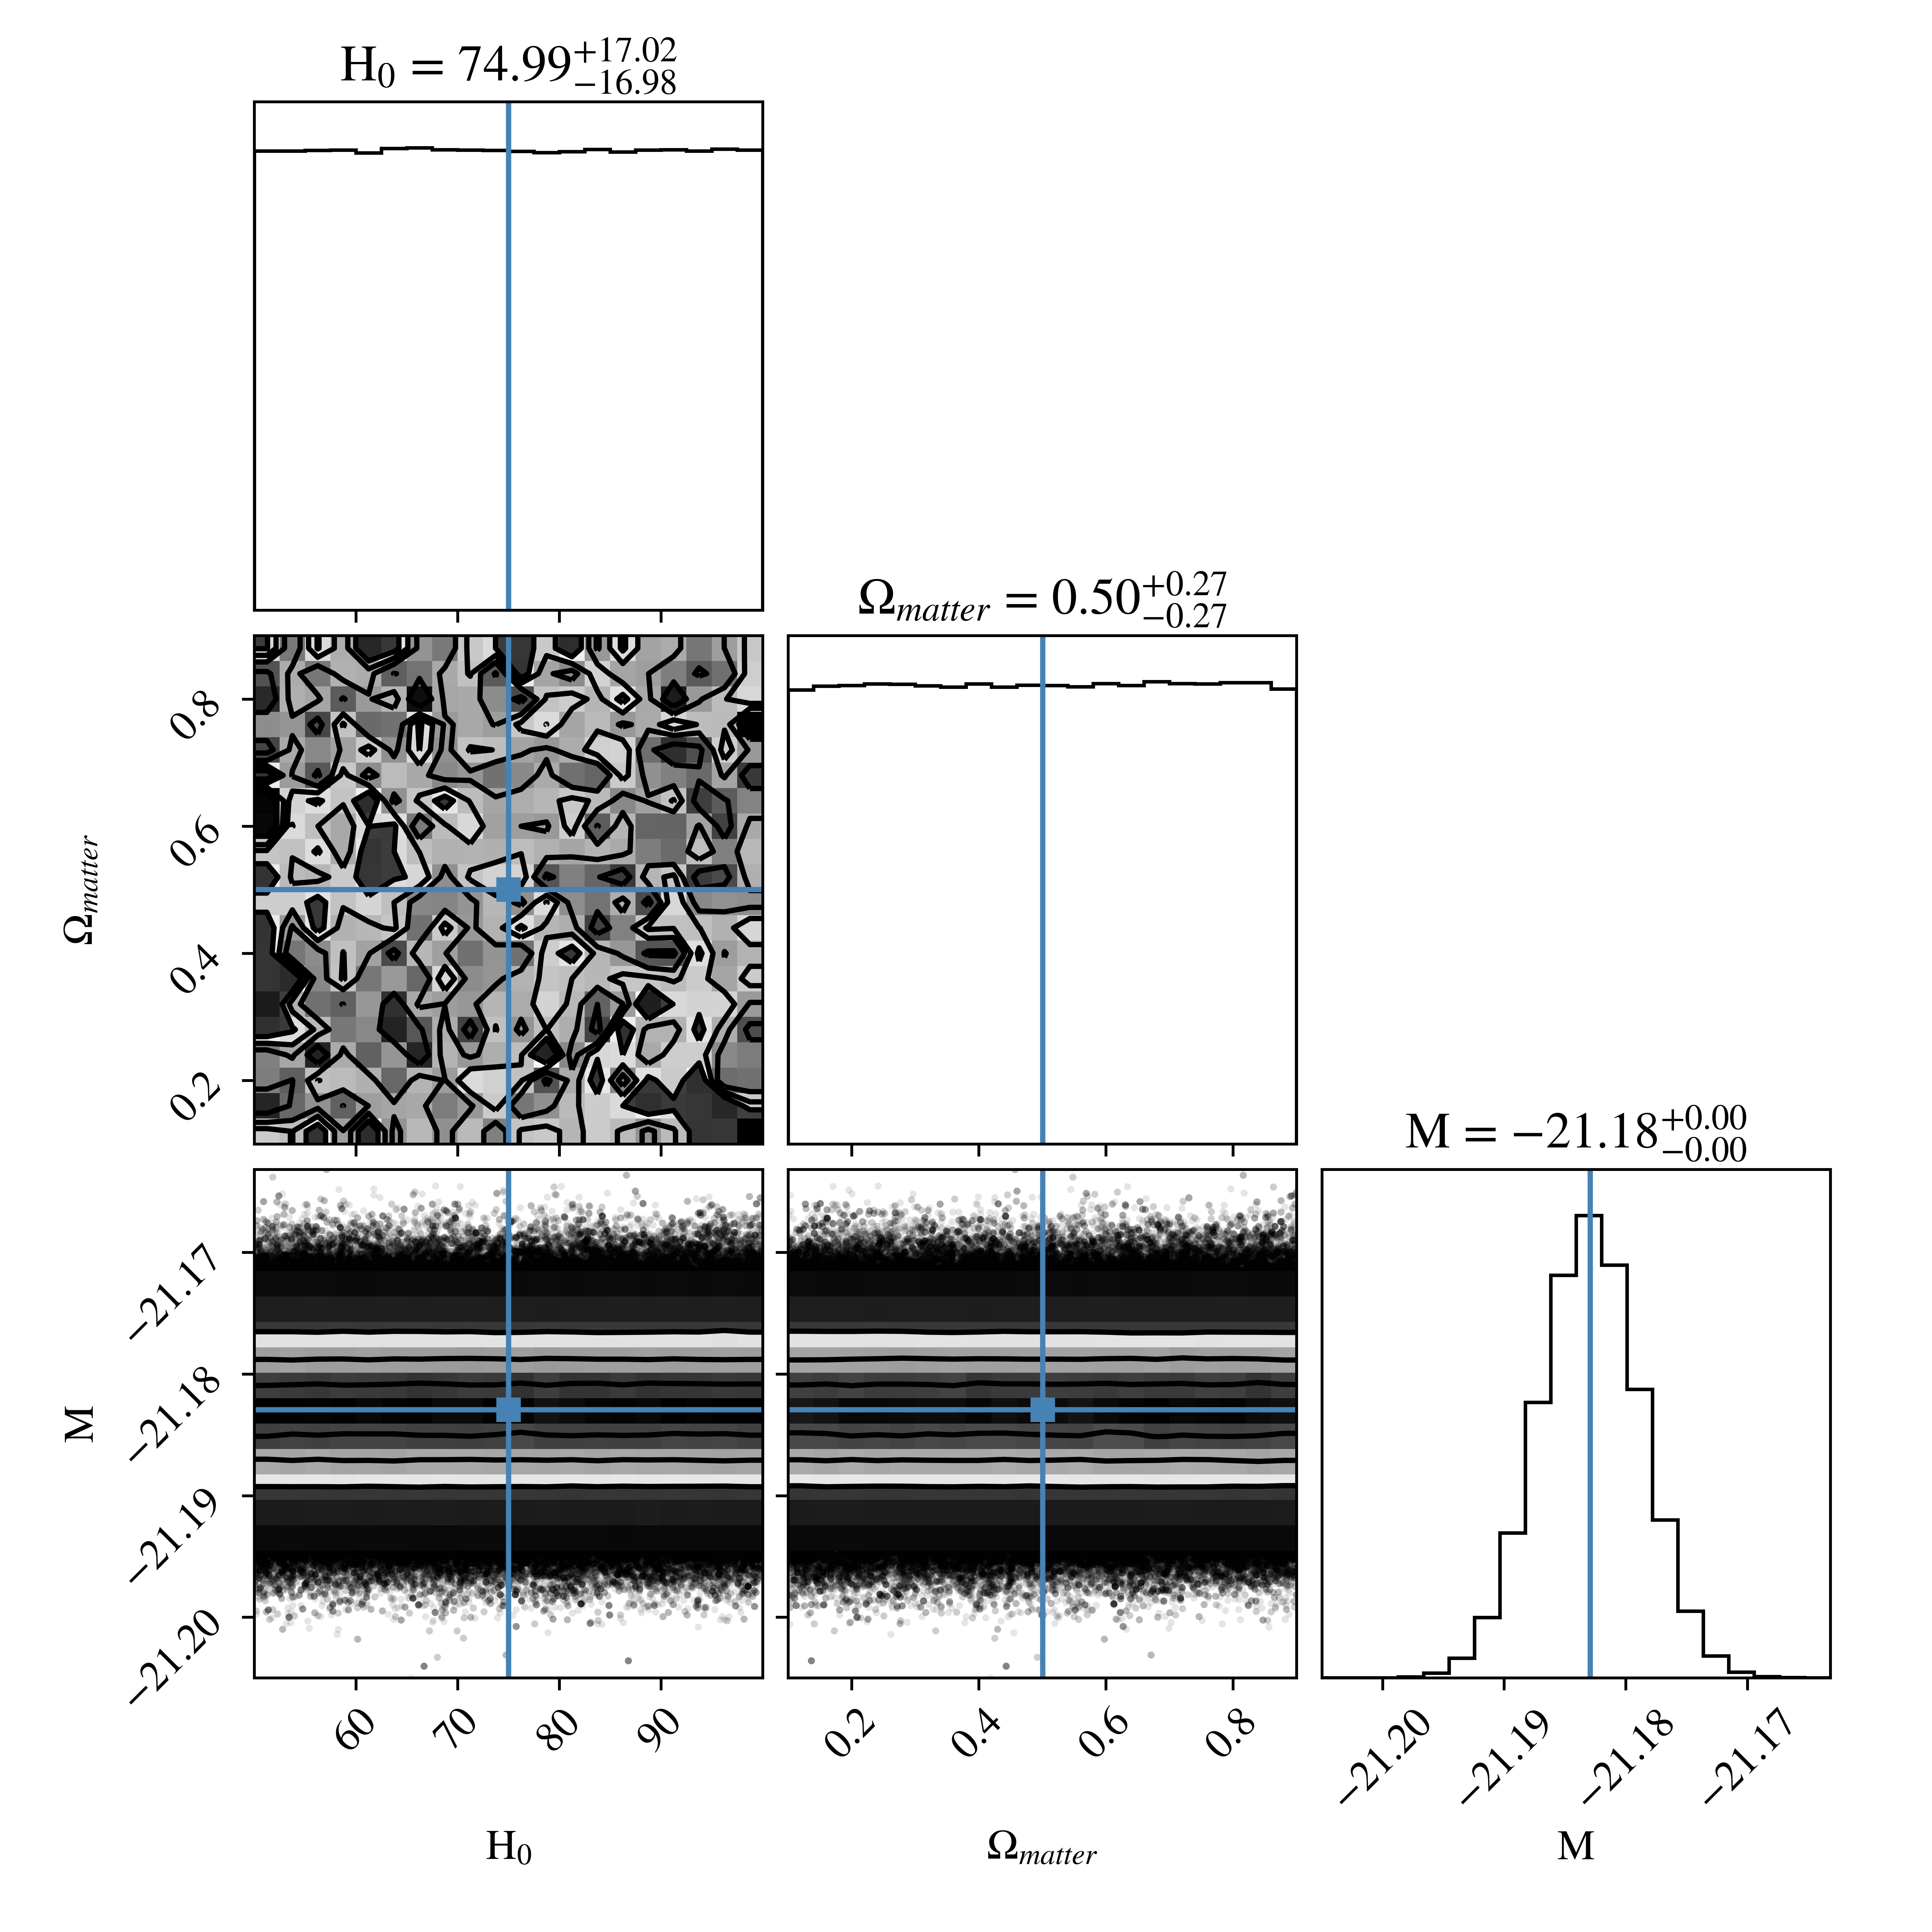
\includegraphics[width = 0.7\textwidth]{Graph 4.png}
    \label{fig:corner~plots}
\end{figure}

From the figure one can note that the best fit parameters were \(H_0\) = \num{74.99 \pm 17.02}\unit{km.s^{-1}.Mpc^{-1}}, \(\Omega_{\mathrm{matter}} = 0.5 \pm 0.27\) and \(M = -21.18\). The points of intersection showed by the blue lines on the corner plots indicate where the best fit parameters can be found. 

\begin{figure}[H]
    \centering
    \includegraphics[width = 0.7\textwidth]{Graph 5.png}
\end{figure}

\section{References}
\printbibliography[heading = none]

\section{Appendix}
\begin{minted}{py}
import numpy as np
import matplotlib.pyplot as plt
import pandas as pd
import batman
import emcee
import corner
from math import *
from sympy import *
from scipy.integrate import romberg
from scipy.optimize import minimize, curve_fit

#Defining the redshift range and other constants to be used
z_range = np.arange(0, 2.4, 0.01)   #redshift range
omega_matter = 0.315                #P18 value for omega_matter
omega_matter_delta = 0.007          #P18 value for the error of omega_matter
H_0 = 67.4                          #P18 value for H_0
H_0_delta = 0.5                     #P18 value for the error of H_0

#Working out the Hubble parameter and its error for each redshift
H_z_list = []
for z in z_range:
  H_z = np.sqrt((H_0**2) * (omega_matter * ((1 + z)**3) + (1 - omega_matter)))  #Hubble parameter
  H_z_list.append(H_z)
  
#Generating the line of best fit using polyfit
coeffs_H, cov = np.polyfit(z_range, H_z_list, 1, cov=True)
poly_function = np.poly1d(coeffs_H)
trendline_H_z = poly_function(z_range)

#Plotting a graph of the Hubble parameter against redshift
plt.figure(figsize=(7.5, 10.5))
plt.rcParams['font.family'] = 'STIXGeneral'
plt.rcParams['mathtext.fontset'] = 'stix'
plt.rcParams['font.size'] = 12
plt.rcParams['font.weight'] = 'normal'
plt.minorticks_on()
plt.grid(visible=True, which='major', linestyle='-')
plt.grid(visible=True, which='minor', linestyle='--')
plt.scatter(z_range, H_z_list, color = 'k')
plt.plot(z_range, trendline_H_z, color ='k')
plt.xlabel(r'z / km s$^{-1}$')
plt.ylabel(r'H(z) / km s$^{-1}$ Mpc$^{-1}$')
plt.title('A graph of H(z) against z')
plt.tight_layout()
plt.savefig('Graph 1.png', dpi=800)
plt.show()

#Defining the constant to be used
c = 299792.458    #speed of light

#Working out the luminosity distance for each redshift using the integrate.romberg numerical integrator
luminosity_list =[]
dL = []
for i in range(len(z_range)):
  dl_func = lambda dl: (2 * np.sqrt(((omega_matter) * ((1 + z_range[i]) ** 3)) + ((H_0) * (1-omega_matter)))) / ((3 * (H_0 ** 2) * omega_matter) + (6 * (H_0 ** 2) * omega_matter * z_range[i]) + (3 * (H_0 ** 2) * omega_matter * (z_range[i] ** 2)))    #first derivative of the Hubble parameter wrt z
  luminosity = romberg(dl_func, 0, 2.3)           #integration of the first derivative of the Hubble parameter from 0 to z
  luminosity_list.append(luminosity)
  const = c * (1 + z_range[i])                        #constant
  luminosity = float(luminosity_list[i]) * const    #luminosity distance
  dL.append(luminosity)

#Plotting a graph of the luminosity distance against redshift
plt.figure(figsize=(7.5, 10.5))
plt.rcParams['font.family'] = 'STIXGeneral'
plt.rcParams['mathtext.fontset'] = 'stix'
plt.rcParams['font.size'] = 12
plt.rcParams['font.weight'] = 'normal'
plt.minorticks_on()
plt.grid(visible=True, which='major', linestyle='-')
plt.grid(visible=True, which='minor', linestyle='--')
plt.scatter(z_range, dL, color='k')
plt.xlabel(r'z / km s$^{-1}$')
plt.ylabel(r'd$_L$ / pc')
plt.title(r'A graph of d$_L$ against z')
plt.tight_layout()
plt.savefig('Graph 2.png', dpi=800)
plt.show()

#Using pandas to load the SN data set
df = pd.read_excel('lcparams.xlsx')
redshift = df['zcmb']   #redshift in the rest frame of the cosmic microwave background radiation
dm = df['mb']           #distance modulus
delta_dm = df['dmb']    #error of the distance modulus

#Plotting a graph of the distance modulus, and its uncertainty, against redshift of the SN data set
plt.figure(figsize=(7.5, 10.5))
plt.rcParams['font.family'] = 'STIXGeneral'
plt.rcParams['mathtext.fontset'] = 'stix'
plt.rcParams['font.size'] = 12
plt.rcParams['font.weight'] = 'normal'
plt.minorticks_on()
plt.grid(visible=True, which='major', linestyle='-')
plt.grid(visible=True, which='minor', linestyle='--')
plt.errorbar(redshift, dm, xerr=0, yerr=delta_dm, fmt='o', color='k', elinewidth=2, capthick=2, capsize=5, ecolor='grey')
plt.xlabel(r'redshift$_{SN}$')
plt.ylabel(r'$\mathrm{\mu}_{SN}$')
plt.title(r'A graph of $\mathrm{\mu}_{SN}$ against redshift$_{SN}$')
plt.tight_layout()
plt.savefig('Graph 3.png', dpi=800)
plt.show()

#Implementing a general purpose MCMC from the emcee library to find the best fit theta parameters

#Working out the luminosity distance for each redshift using the P18 values and the integrate.romberg numerical integrator
def dL_func(z, H_0, omega):
  for i in range(len(redshift)):
    dl_func = lambda dl: (2 * np.sqrt(((omega_matter) * ((1 + z_range[i]) ** 3)) + ((H_0) * (1 - omega_matter)))) / ((3 * (H_0 ** 2) * omega_matter) + (6 * (H_0 ** 2) * omega_matter * z_range[i]) + (3 * (H_0 ** 2) * omega_matter * (z_range[i] ** 2)))
    luminosity = romberg(dl_func, 0, 2.3)
    luminosity_list.append(luminosity)
    const = c * (1 + z_range[i])
    luminosity = float(luminosity_list[i]) * const
    return luminosity

#Working out the model distance modulus for each redshift using the dL_func and the P18 values
def model(theta, x=redshift):
    H_0, omega_matter, M = theta
    for i in range(len(redshift)):
      dL_model = dL_func(redshift[i], H_0, omega_matter)
      model = (5) * (np.log10(dL_model)) + 25 + M
      return model

#Setting the observed distance modulus for each redshift using the SN data set
def observed(theta, x=redshift):
    H_0, omega_matter, M = theta
    observed = dm
    return observed

#Calculating the likeliness of fit of the theta parameters to the SN data set
def like(theta, x=redshift, y=dm, yerr=delta_dm):
    H_0, omega_matter, M = theta
    model2 = model(theta, x=redshift)
    observed2 = observed(theta, x=redshift)
    like = (-0.5)*(np.sum(((model2-observed2)**2)/(yerr)**2))
    return like

#Setting the priors of the theta parameters then calling the function at every step to check if all arguments are within their respective priors
def prior(theta):
    H_0, omega_matter, M = theta
    if 50 < H_0 < 100 and 0.1 < omega_matter < 0.9 and -50 < M < 50:
        return 0
    else:
        return -np.inf

#Calling the prior function to check if it returns -infinity or 0, and returning -infinity or the likelihood function for the theta parameters in each respective case
def probability(theta, x=redshift, y=dm, yerr=delta_dm):
    prob = prior(theta)
    if not np.isfinite(prob):
        return -np.inf
    return prob + like(theta, x=z_range, y=dm, yerr=delta_dm)

#Defining a tuple with the SN data set
data = (redshift, dm, delta_dm)
#Setting the number of walkers
n_walkers = 100
#Setting the number of iterations
n_iter = 60000
#Setting an array with the initial positions
initial = np.array([70, 0.3, -19])
#Setting the dimension
n_dim = len(initial)

#Calculating the step methodology across the parameter space from one place of the grid to the next
def p_0(initial, n_dim, n_walkers):
      return [np.array(initial) + [1e-4, 75e-3, 1e-2] * np.random.randn(n_dim) for i in range(n_walkers)]

p0 = p_0(initial, n_dim, n_walkers)

#Defining and implementing the MCMC
def mcmc(p0, n_walkers, n_iter, n_dim, probability, data):
    sampler = emcee.EnsembleSampler(n_walkers, n_dim, probability, args=[data])
    print('Running sample run')
    p0, _, _ = sampler.run_mcmc(p0, 2000, progress=True)
    sampler.reset()
    print('Running full mcmc')
    posteriors, probability, state = sampler.run_mcmc(p0, n_iter, progress=True)
    return sampler, posteriors, probability, state

sampler, posteriors, probability, state = mcmc(p0, n_walkers, n_iter, n_dim, probability, data)

#Flattening the outputted samples to be able to plot a corner plot with the outputted theta parameters
samples = sampler.flatchain

#Calculating the mean values of the outputted theta parameters
mean_H_0 = np.mean(samples[:,0])
mean_omega = np.mean(samples[:,1])
mean_M = np.mean(samples[:,2])

#Plotting a corner plot with the outputted theta parameters
labels = [r'H$_{0}$', '$\mathrm{\Omega}_{matter}$', 'M']
fig = corner.corner(samples, show_titles=True, labels=labels, truths=[mean_H_0, mean_omega, mean_M])
plt.savefig('Graph 4.png', dpi=800)

lum = []
for z in redshift:
  #Working out the Hubble parameter for each redshift using the mean values of the outputted theta parameters
  Hz = np.sqrt((mean_H_0**2) * (mean_omega * ((1 + z)**3) + (1 - mean_omega)))
  #Working out the luminosity distance for each redshift using the mean values of the outputted theta parameters and the integrate.romberg numerical integrator
  dl_func = lambda dl: (2 * np.sqrt(((mean_omega) * ((1 + z) ** 3)) + ((Hz) * (1 - mean_omega)))) / ((3 * (Hz ** 2) * mean_omega) + (6 * (Hz ** 2) * mean_omega * z)+(3 * (Hz ** 2) * mean_omega * (z ** 2)))
  luminosity = romberg(dl_func, min(redshift), max(redshift))
  const = c * (1 + z)
  lum.append(const*float(luminosity))

#Fitting the outputted theta parameters to the SN data set
def fit_func(lum, mean_M):
  return (5) * (np.log10(lum)) + 25 + mean_M

#Generating the line of best fit using curve_fit
popt, pcov = curve_fit(fit_func, redshift, dm)
trendline = fit_func(redshift, popt[0])

#Plotting the result of the fit superimposed on the original graph of the distance modulus, and its uncertainty, against redshift of the SN data set
plt.figure(figsize=(7.5, 10.5))
plt.rcParams['font.family'] = 'STIXGeneral'
plt.rcParams['mathtext.fontset'] = 'stix'
plt.rcParams['font.size'] = 12
plt.rcParams['font.weight'] = 'normal'
plt.minorticks_on()
plt.grid(visible=True, which='major', linestyle='-')
plt.grid(visible=True, which='minor', linestyle='--')
plt.errorbar(redshift, dm, xerr=0, yerr=delta_dm, fmt='o', color='k', elinewidth=2, capthick=2, capsize=5, ecolor='grey')
plt.plot(redshift, trendline, '--', label='Fit')
plt.xlabel(r'redshift$_{SN}$')
plt.ylabel(r'$\mathrm{\mu}_{SN}$')
plt.title(r'A graph of $\mathrm{\mu}_{SN}$ against redshift$_{SN}$')
plt.legend()
plt.tight_layout()
plt.savefig('Graph 5.png', dpi=800)
plt.show()
\end{minted}

\end{document}